\section{discussion and conclusion}




In this paper, we propose using the massive collections of
user-generated photos uploaded to social sharing websites as a source
of observational evidence about the world, and in particular as a way
of estimating the presence of ecological phenomena. As a first step
towards this long-term goal, we used a collection of 150 million
geo-tagged, timestamped photos from Flickr to estimate snow 
cover and greenery, and compared these estimates to fine-grained
ground truth collected by earth-observing satellites and ground stations. We compared
several techniques for performing the estimation from noisy, biased
data, including simple voting mechanisms and a Bayesian likelihood
ratio. We also tested several possible improvements to these basic
%%hp cr: removed "multi-language tag sets" as we did not report it in
%%this version
methods, including using 
%temporal smoothing, 
%multi-language tag sets,
machine learning to improve the accuracy of estimates.

In this paper, we show a real case of using public-sharing data to estimate ecology information.
We used get this information only from some institution with the help of satellite.
Also, we propose using photo-sharing social media sites as a
means of observing the state of the natural world, by automatically
recognizing specific types of scenes and objects in large-scale social
image collections. This work is an initial step towards a long-term
goal of monitoring important ecological events and trends through
online social media.  




Our study shows that snowy scene recognition is
not nearly as easy a problem as one might expect, when applied to realistic
consumer images; our best result using
modern vision techniques gives 81\% accuracy. Nevertheless, as a proof-of-concept
we demonstrated that this recognition accuracy still yields a reasonable
map that approximates observations from satellites.
%However, using the current modern vision techniques to solve
%this problem, we are able to recreate the satellite map.  
We also test recognition algorithms on their ability to recognize a
particular species of flower, the California Poppy. In future work, we
plan to combine evidence from tags and other metadata with visual
features for more accurate estimates, and to develop novel techniques
for these challenging recognition problems. 

\fxnote{possible ideas in discussion section}

%0. not using tags in vegetation case
An important work in this paper is analyzing the visual content of image data instead of
only using text tags. The complement information in image content is crucial for some phenomena. For example, in vegetation case, 
%Discussion about the fact that tags really do not work well for some
%phenomena like vegetation where 
there is not a single set of ``good''
tags that all users would use. Many terms, like ``forest'', ``tree'', ``green'' and etc., can point to images with no greenery content.
Further more, it is hard to see much description about the leaves are green or yellow in tags.
And also a lot of tags are misleading such as ``Irish green'' on Saint Patrick's Day. 

%1. wrong case analysis

%a. complex dataset of image classification

%This part probably requires some image examples to show how complex the dataset is and why the 
%image classification cannot be perfect. 
%And images is easily take large space.

The public sharing images we use are not taken on purpose of research work. Instead, users all have their own views of taking photos. That makes our data set very complex in content, viewing angle, and illumination. 
\fxnote{This is a possible factor about 
why our visual image classification model does not perform perfect. Or this is the key challenge of the image classification step.}

To show the diversity of our Flickr image dataset, in figure ~\ref{fig:dataset} we present a random sample of images in our vegetation dataset.
Trees in the images can be far away from camera, or only as a background of another event or object in the scene. In negative set, the images can also be confusing like forests in winter without leaves, or plants in pictures or indoor.

%\begin{figure*}[th]
%{\small{
%\begin{center}
%\begin{tabular}{@{}c@{\,\,\,}c@{\,\,\,}c@{\,\,\,}c@{\,\,\,}c@{\,\,\,}}
%%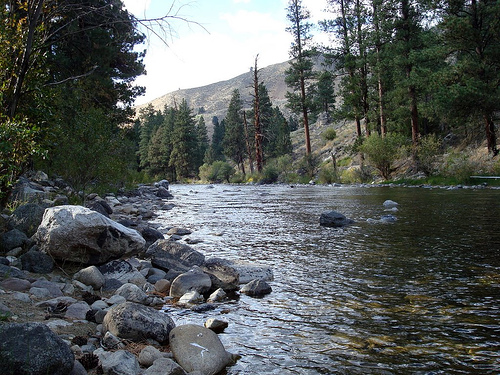
\includegraphics[width=0.19\textwidth]{imggrid/datasetposi/1.jpg} &
%%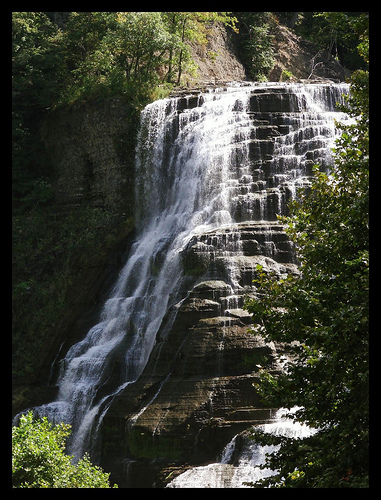
\includegraphics[height=1in]{imggrid/datasetposi/2.jpg} &
%%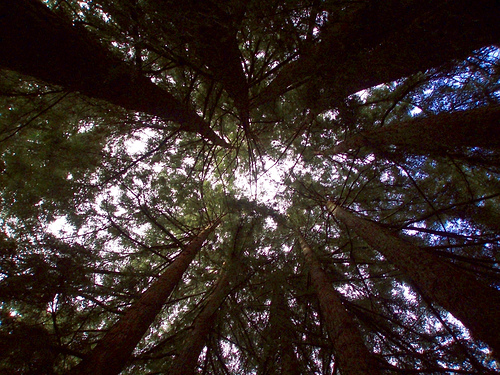
\includegraphics[width=0.19\textwidth]{imggrid/datasetposi/3.jpg} &
%%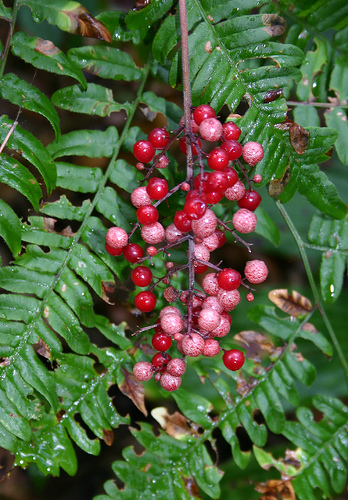
\includegraphics[height=1in]{imggrid/datasetposi/4.jpg} &
%%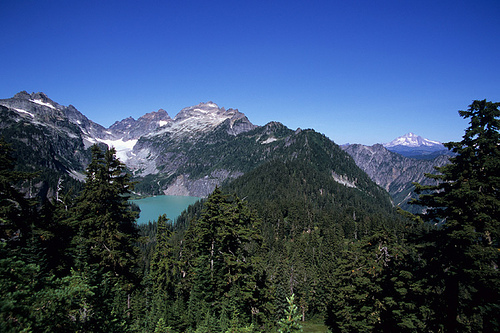
\includegraphics[width=0.19\textwidth]{imggrid/datasetposi/5.jpg} \\
%%%\multicolumn{5}{c}{(a) Random positive images in vegetation dataset} \\
%%\\[-6pt]
%%\hline
%%\\[-6pt]
%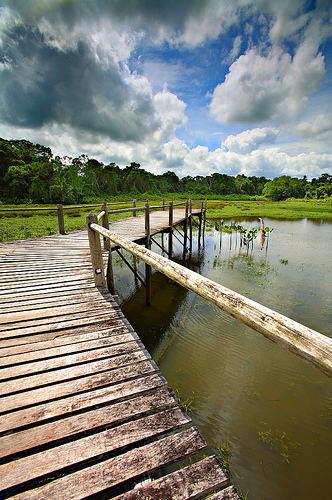
\includegraphics[height=1in]{imggrid/datasetposi/6.jpg} &
%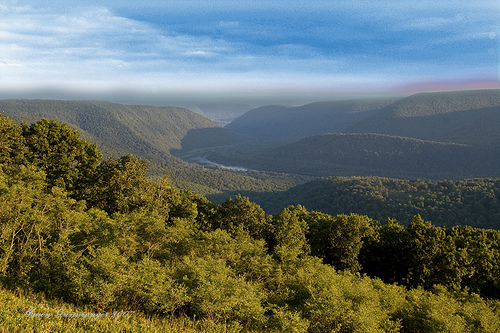
\includegraphics[width=0.19\textwidth]{imggrid/datasetposi/7.jpg} &
%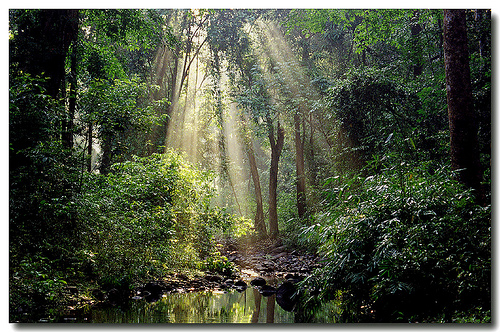
\includegraphics[width=0.19\textwidth]{imggrid/datasetposi/8.jpg} &
%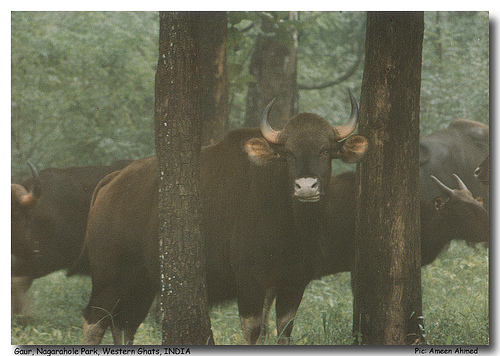
\includegraphics[width=0.19\textwidth]{imggrid/datasetposi/9.jpg} &
%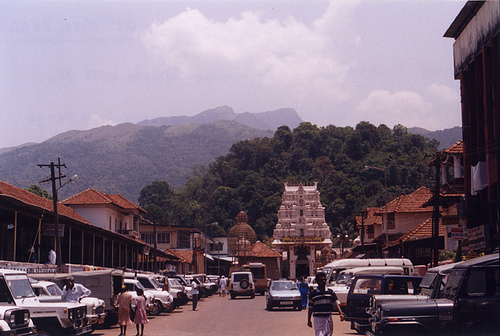
\includegraphics[width=0.19\textwidth]{imggrid/datasetposi/10.jpg} \\
%\multicolumn{5}{c}{(a) Random positive images in vegetation dataset} \\ 
%\\[-6pt]
%\hline
%\\[-6pt]
%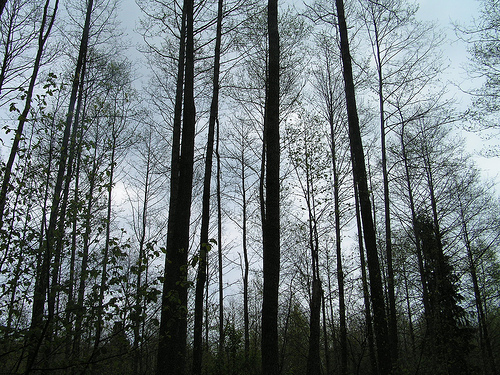
\includegraphics[width=0.19\textwidth]{imggrid/datasetnega/1.jpg} &
%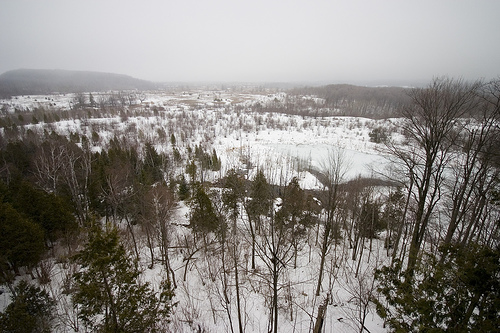
\includegraphics[width=0.19\textwidth]{imggrid/datasetnega/2.jpg} &
%%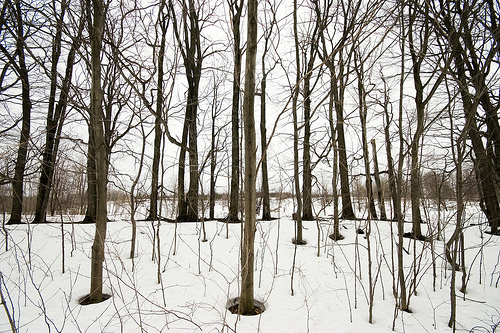
\includegraphics[width=0.19\textwidth]{imggrid/datasetnega/3.jpg} &
%%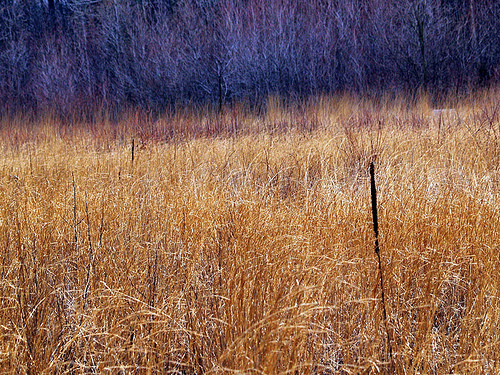
\includegraphics[width=0.19\textwidth]{imggrid/datasetnega/4.jpg} &
%%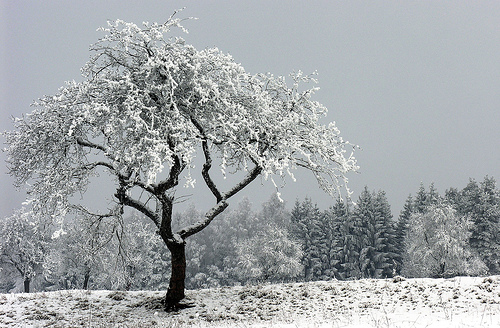
\includegraphics[width=0.19\textwidth]{imggrid/datasetnega/5.jpg} \\
%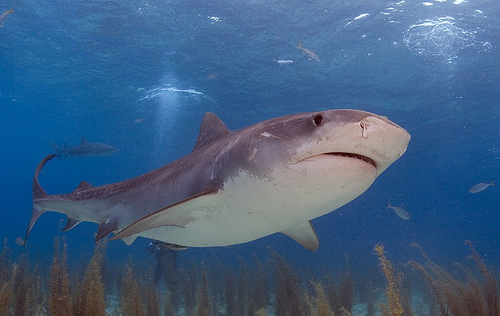
\includegraphics[width=0.19\textwidth]{imggrid/datasetnega/7.jpg} &
%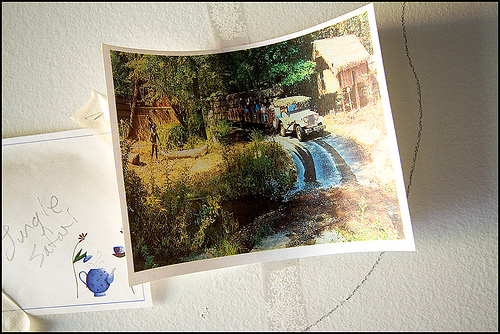
\includegraphics[width=0.19\textwidth]{imggrid/datasetnega/8.jpg} &
%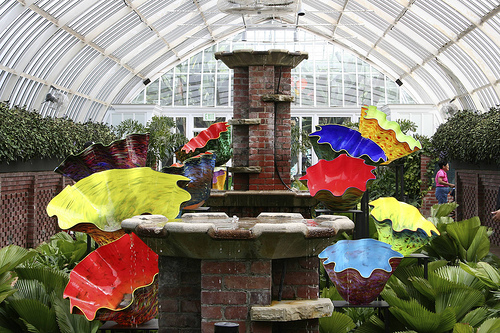
\includegraphics[width=0.19\textwidth]{imggrid/datasetnega/10.jpg} \\
%%\multicolumn{5}{c}{(c) Random false negatives (snow images classified as non-snow)} \\ 
%%\\[-6pt]
%%\hline
%%\\[-6pt]
%%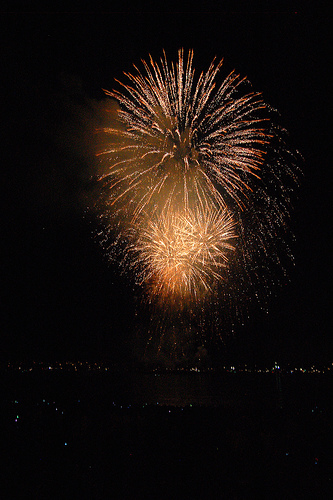
\includegraphics[height=1in]{imggrid/datasetnega/6.jpg} &
%%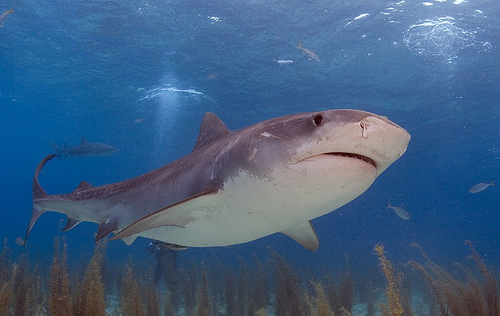
\includegraphics[width=0.19\textwidth]{imggrid/datasetnega/7.jpg} &
%%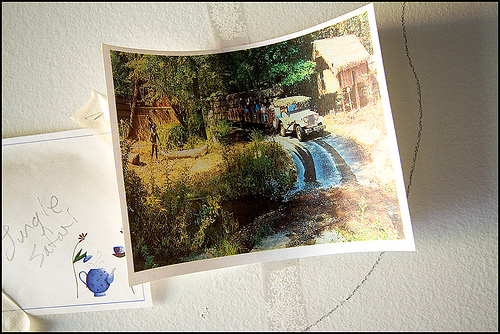
\includegraphics[width=0.19\textwidth]{imggrid/datasetnega/8.jpg} &
%%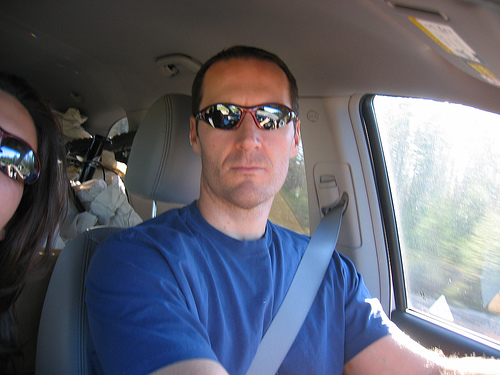
\includegraphics[width=0.19\textwidth]{imggrid/datasetnega/9.jpg} &
%%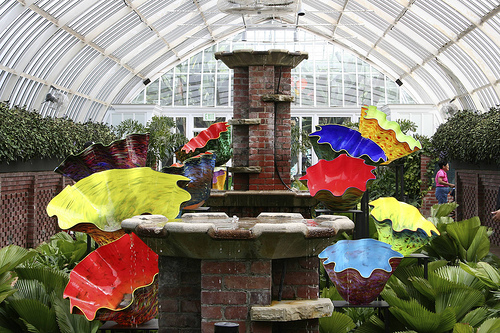
\includegraphics[width=0.19\textwidth]{imggrid/datasetnega/10.jpg} \\
%\multicolumn{5}{c}{(b) Random negative images in vegetation dataset} \\
%\end{tabular}
%\end{center}
%}}
%\caption{Random images from our hand-labeled dataset. Public sharing images are various in quality, contents, illumination and view angle.
%Negative images like winter trees without leaves, or indoor images capturing a photo of forest are more confusing.}
%\label{fig:dataset}
%\end{figure*}

\begin{figure}[th]
{\small{
\begin{center}
\begin{tabular}{@{}c@{\,\,\,}c@{\,\,\,}c@{\,\,\,}c@{\,\,\,}c@{\,\,\,}}
\vspace{10pt}
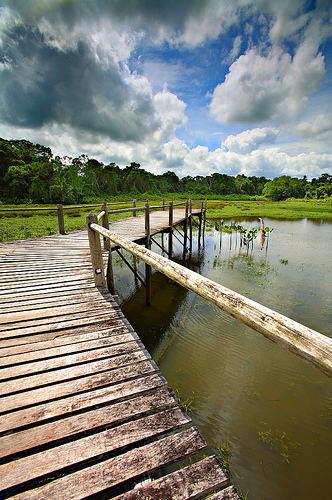
\includegraphics[height=0.5in]{imggrid/datasetposi/6.jpg} &
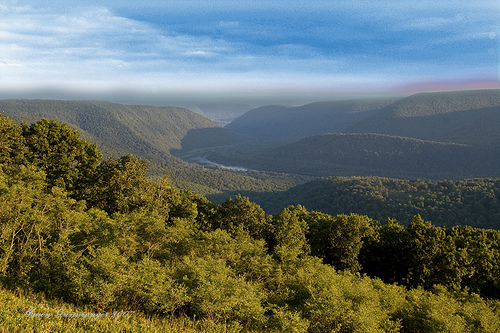
\includegraphics[width=0.08\textwidth]{imggrid/datasetposi/7.jpg} &
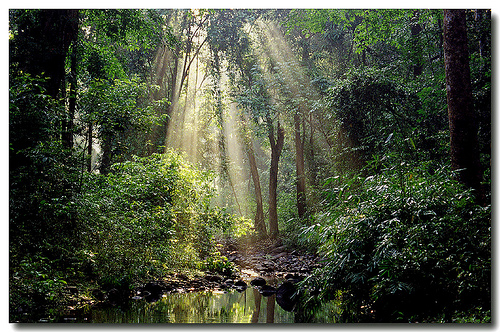
\includegraphics[width=0.08\textwidth]{imggrid/datasetposi/8.jpg} &
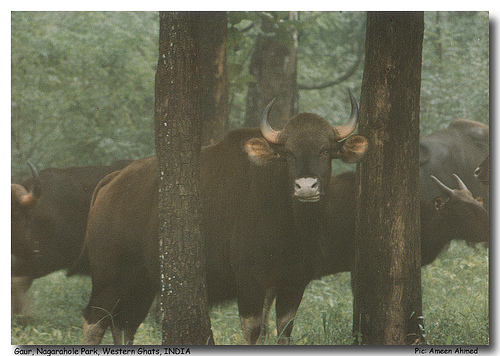
\includegraphics[width=0.08\textwidth]{imggrid/datasetposi/9.jpg} &
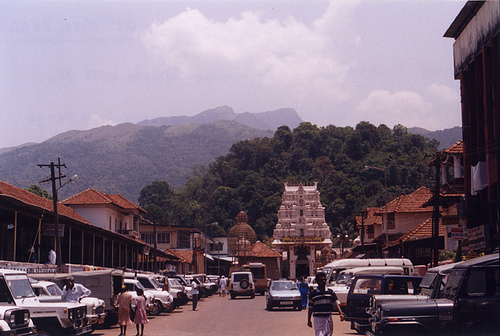
\includegraphics[width=0.08\textwidth]{imggrid/datasetposi/10.jpg} \\
\multicolumn{5}{c}{(a) Random positive images in vegetation dataset} \\
\\[-6pt]
\hline
\\[-6pt]
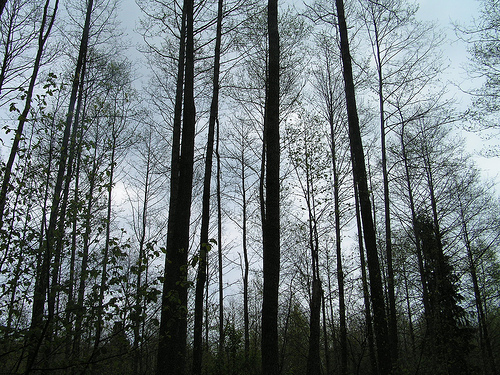
\includegraphics[width=0.08\textwidth]{imggrid/datasetnega/1.jpg} &
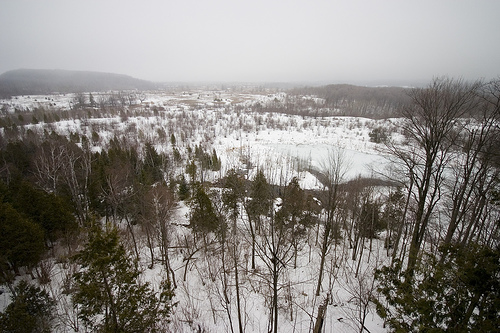
\includegraphics[width=0.08\textwidth]{imggrid/datasetnega/2.jpg} &
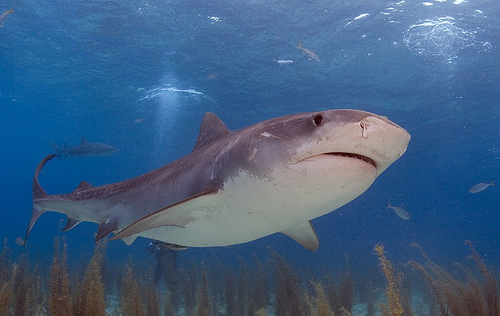
\includegraphics[width=0.08\textwidth]{imggrid/datasetnega/7.jpg} &
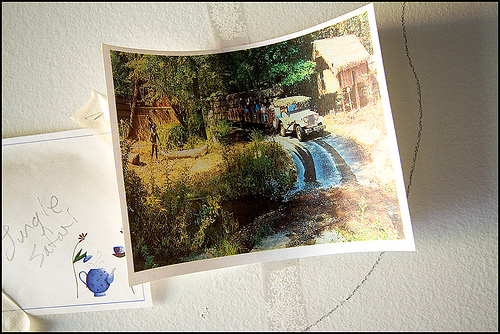
\includegraphics[width=0.08\textwidth]{imggrid/datasetnega/8.jpg} &
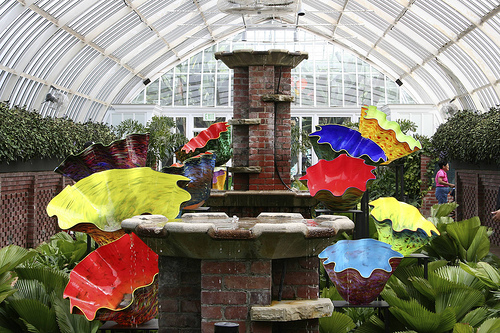
\includegraphics[width=0.08\textwidth]{imggrid/datasetnega/10.jpg} \\
\multicolumn{5}{c}{(b) Random negative images in vegetation dataset} \\
\end{tabular}
\end{center}
}}
\caption{Random images from our hand-labeled dataset. Public sharing images are various in quality, contents, illumination and view angle.
Negative images like winter trees without leaves, or indoor images capturing a photo of forest are more confusing.}
\label{fig:dataset}
\end{figure}

%b. wrong case of bin prediction

In continental scale prediction, from the non-green bins in ground truth, we find a lot of 
green images from our dataset.
%This part is now in results section. We can move it to discussion section if necessary.
\fxnote{
It is possible that within the $50 km$ by $50 km$ bin, 
there are greenery in small region but not large enough to 
cover 50\% of the land. It is also possible that 
the satellite does not detect more than 50\% of greenery because of cloud coverage. 
(I do not believe what I wrote... We've kicked out bins with high cloud coverage. 
I cannot explain this)
}

%2. deep learning performs better than visual features

Our experiments also provide evidence for the latest improvement in image classification -- CNN outperforms traditional vision technique when
 we have a large number of training data. The reason is not completely understood. And we only 
discuss our speculation here.
Intuitively, deep learning technique learns very high dimensional features in hierarchy way from training data
while traditional methods directly extract hand designed visual features. Also CNN achieves 
global optimization with feature
learning and classification. In traditional methods, instead, feature extraction and image
classification perform separately.



%3. future works
In future, we have some plans to build a more sophisticated system.
The vegetation coverage changes at different time over places. 
Instead of trying to create a single binary classifier (to determine whether this image is with or
without a certain ecology phenomenon),
we can train individual classifiers on one particular place 
-- e.g. Eiffel tower, etc. 
In this way, we will be able to 
take advantage of the static landmark and make a more accurate image classification model.

%Instead of trying to create a single snow vs non-snow 
%(or green vs non-green, or whatever), 
%instead train individual classifiers trained on one particular place 
%-- e.g. Eiffel tower, etc. 
%This could also use 3d models like in the Snavely ECCV 2014 paper, 
% but that might not be needed.

We also plan to build a super tiny image from all the images we collect from each location at each time period. 
These images make a video visualization of how the vegetation coverage changes over time in North American continent.

\fxnote{Sorry I do not understand this well enough}
Look at time series of photos at a single place across time 

More generally, we hope
the idea of observing nature through photo-sharing websites will help
spark renewed interest in recognizing natural and ecological phenomenon in
consumer images.
%=======
%In this paper, we   propose using massive amount of latent visual information uploaded to social media as source  observing the state of the natural world by recognizing specific types of scenes and objects in large-scale social image collections. This work can be considered as  preliminary step towards long-term goal to understand the ecology phenomena using online social media.  Our study shows that snowy scene recognition  is not an easy problem as been expected. Best  results obtained using modern vision techniques is around 81\% accuracy which is not  high accuracy. However, using  the current modern vision techniques to solve this problem, we are able to recreate the satellite map.  We also  show the   current  recognition algorithms able to  detect a particular species of flower, the California
%Poppy at accuracy 72\%. 
%In future work we plan to find more sophisticated computer vision techniques for  these problems. Also, we plan to combine this work  with  the work of Zhang \textit{et al}~\cite{ecology2012www} which is based on textual information to improve the results. Also, we plan to study more ecological phenomena like migration patterns of wildlife.
%>>>>>>> .r2693

%% In future work we plan to find more sophisticated computer vision
%% techniques for these problems. Also, we plan t combine this work based
%% on visual information with the work of Zhang \textit{et
%%   al}~\cite{ecology2012www} which is based on textual information to
%% improve the results. Also, we plan to study more ecological phenomena
%% like migration patterns of wildlife.


 
%We found
%that while the recall is relatively low due to the sparsity of photos
%on any given day, the precision can be quite high, suggesting that
%mining from photo sharing websites could be a reliable source of
%observational data for ecological and other scientific research. 
%In
%future work, we plan to study additional features including using
%more sophisticated computer vision techniques to analyze visual content. Also we plan to study a variety of other ecological phenomena,
%including those for which high quality ground truth is not available,
%such as migration patterns of wildlife and the distributions of
%blooming flowers.






% if have a single appendix:
%\appendix[Proof of the Zonklar Equations]
% or
%\appendix  % for no appendix heading
% do not use \section anymore after \appendix, only \section*
% is possibly needed

% use appendices with more than one appendix
% then use \section to start each appendix
% you must declare a \section before using any
% \subsection or using \label (\appendices by itself
% starts a section numbered zero.)
%



